%\documentclass[twocolumn,journal]{IEEEtran}
\documentclass[onecolumn,journal]{IEEEtran}
\usepackage{amsfonts}
\usepackage{amsmath}
\usepackage{amsthm}
\usepackage{amssymb}
\usepackage{graphicx}
\usepackage[T1]{fontenc}
%\usepackage[english]{babel}
\usepackage{supertabular}
\usepackage{longtable}
\usepackage[usenames,dvipsnames]{color}
\usepackage{bbm}
%\usepackage{caption}
\usepackage{fancyhdr}
\usepackage{breqn}
\usepackage{fixltx2e}
\usepackage{capt-of}
%\usepackage{mdframed}
\setcounter{MaxMatrixCols}{10}
\usepackage{tikz}
\usetikzlibrary{matrix}
\usepackage{endnotes}
\usepackage{soul}
\usepackage{marginnote}
%\newtheorem{theorem}{Theorem}
\newtheorem{lemma}{Lemma}
%\newtheorem{remark}{Remark}
%\newtheorem{error}{\color{Red} Error}
\newtheorem{corollary}{Corollary}
\newtheorem{proposition}{Proposition}
\newtheorem{definition}{Definition}
\newcommand{\mathsym}[1]{}
\newcommand{\unicode}[1]{}
\newcommand{\dsum} {\displaystyle\sum}
\hyphenation{op-tical net-works semi-conduc-tor}
\usepackage{pdfpages}
\usepackage{enumitem}
\usepackage{multicol}
\usepackage[sort&compress]{natbib}

\headsep = 5pt
\textheight = 730pt
%\headsep = 8pt %25pt
%\textheight = 720pt %674pt
%\usepackage{geometry}

\bibliographystyle{unsrt}

\usepackage{float}

\usepackage{xcolor}
 
\usepackage[framemethod=TikZ]{mdframed}
%%%%%%%FRAME%%%%%%%%%%%
\usepackage[framemethod=TikZ]{mdframed}
\usepackage{framed}
    % \BeforeBeginEnvironment{mdframed}{\begin{minipage}{\linewidth}}
     %\AfterEndEnvironment{mdframed}{\end{minipage}\par}
% \usepackage[document]{ragged2e}

%	%\mdfsetup{%
%	%skipabove=20pt,
%	nobreak=true,
%	   middlelinecolor=black,
%	   middlelinewidth=1pt,
%	   backgroundcolor=purple!10,
%	   roundcorner=1pt}

\mdfsetup{%
	outerlinewidth=1,skipabove=20pt,backgroundcolor=yellow!50, outerlinecolor=black,innertopmargin=0pt,splittopskip=\topskip,skipbelow=\baselineskip, skipabove=\baselineskip,ntheorem,roundcorner=5pt}

\mdtheorem[nobreak=true,outerlinewidth=1,%leftmargin=40,rightmargin=40,
backgroundcolor=yellow!50, outerlinecolor=black,innertopmargin=0pt,splittopskip=\topskip,skipbelow=\baselineskip, skipabove=\baselineskip,ntheorem,roundcorner=5pt,font=\itshape]{result}{Result}


\mdtheorem[nobreak=true,outerlinewidth=1,%leftmargin=40,rightmargin=40,
backgroundcolor=yellow!50, outerlinecolor=black,innertopmargin=0pt,splittopskip=\topskip,skipbelow=\baselineskip, skipabove=\baselineskip,ntheorem,roundcorner=5pt,font=\itshape]{theorem}{Theorem}

\mdtheorem[nobreak=true,outerlinewidth=1,%leftmargin=40,rightmargin=40,
backgroundcolor=gray!10, outerlinecolor=black,innertopmargin=0pt,splittopskip=\topskip,skipbelow=\baselineskip, skipabove=\baselineskip,ntheorem,roundcorner=5pt,font=\itshape]{remark}{Remark}

\mdtheorem[nobreak=true,outerlinewidth=1,%leftmargin=40,rightmargin=40,
backgroundcolor=pink!30, outerlinecolor=black,innertopmargin=0pt,splittopskip=\topskip,skipbelow=\baselineskip, skipabove=\baselineskip,ntheorem,roundcorner=5pt,font=\itshape]{quaestio}{Quaestio}

\mdtheorem[nobreak=true,outerlinewidth=1,%leftmargin=40,rightmargin=40,
backgroundcolor=yellow!50, outerlinecolor=black,innertopmargin=5pt,splittopskip=\topskip,skipbelow=\baselineskip, skipabove=\baselineskip,ntheorem,roundcorner=5pt,font=\itshape]{background}{Background}

%TRYING TO INCLUDE Ppls IN TOC
\usepackage{hyperref}


\begin{document}
\title{\color{Brown} Breaking the Testing Logjam: CT scan diagnosis \\
\vspace{-0.35ex}}
\author{Chen Shen, Yaneer Bar-Yam \\ New England Complex Systems Institute \\
 \today 
  \vspace{-14ex} \\ 

   
\bigskip
\bigskip

\textbf{}
 }
    
\maketitle


\flushbottom % Makes all text pages the same height

%\maketitle % Print the title and abstract box

%\tableofcontents % Print the contents section

\thispagestyle{empty} % Removes page numbering from the first page

%----------------------------------------------------------------------------------------
%	ARTICLE CONTENTS
%----------------------------------------------------------------------------------------

%\section*{Introduction} % The \section*{} command stops section numbering

%\addcontentsline{toc}{section}{\hspace*{-\tocsep}Introduction} % Adds this section to the table of contents with negative horizontal space equal to the indent for the numbered sections

%\tableofcontents 
%\section{ Introduction}
\renewcommand{\thefootnote}{\fnsymbol{footnote}}


\begin{multicols}{2}
To contain the spread of the COVID-19 epidemic, early detection and isolation are essential in a country's prevention strategy. In order to for this to be effective, we have to know who are infected by coronavirus as soon as possible. Currently laboratory RT-PCR tests are the predominant method in the majority of countries. Yet these tests suffer from 3 drawbacks:
\begin{itemize}
    \item Long report time. Sampling and testing are usually in geographically separated locations (point of care systems are being introduced but do not yet have the capacity for large scale screening)
    \item Significantly high false-negative rate and sensitivity issues. Some manifestly ill patients have to test several times to get a positive result \cite{PCR-1, PCR-2}
    \item Limited in quantity, they are prioritized to moderate/severe cases. However mild, or even asymptomatic cases, are also contagious. Large scale testing is needed because mild symptoms may be positive for 1 in 25 cases. 
\end{itemize}

These drawbacks lead to a deadlock: because testing capacity is limited, many infected individuals cannot get tested and therefore isolated/treated. By policy they are often being sent home. Even when isolated, they may continue to be infectious after symptoms clear and whether they continue to be infectious is also not being tested. Because many such infectious individuals are in the society, they infect more people and lead to overwhelming the testing capacity as well as medical facilities and the cost in lives and economic activity. 

Thus, without capacity for testing, the policy being adopted runs counter to the ability to contain the disease. 

One way to break free from this deadlock is the assistance from CT imaging.  COVID-19 patients have characteristic features, like multifocal patchy shadows or ground-glass opacities, in chest image even for asymptomatic cases. CT scanners are an existing resource in medical systems, and CT results can be obtained within 15 minutes. The use of CT for pre-screen of diagnosis, can expand testing capacity dramatically. 

This approach was extensively used in Hubei province in China \cite{CT1,CT2,CT3} as an integral part of the early identification and isolation policy that led to a rapid decrease in the number of cases so much so that the lock down has been lifted. CT scans were an integral part of the effort from early case identification throughout the disease progression. Even before or just after mild symptoms the glassy signature is visible and served as a key test to identify cases. Moreover, some cases progressed very far without usual symptoms and the progression was visible on the CT scan. While CT scans may not always distinguish from other lung disease, confirmatory RT-PCR can be used, and in areas of high prevalence this is not a significant limitation.

A just published ``Multinational Consensus Statement'' on the use of chest imaging for COVID-19 \cite{use} gives exactly the opposite recommendation. Its first summary point is ``Imaging is not indicated in patients with suspected COVID-19 and mild clinical features unless they are at risk for disease progression''. Remarkably, the one Chinese collaborator is from Sichuan province, which had a maximum of 35 cases per day, far from the outbreak in Wuhan. Buried in this paper is the statement ``The greater sensitivity of CT [compared to chest X-ray] for early pneumonic changes is more relevant in the setting of a public health approach that required isolation of all infected patients within an environment where the reliability of COVID-19 testing was limited and turnaround times were long.'' This is precisely the need in the US and Europe in areas where PCR testing is insufficient and public health prevention is critical. The policy of sending individuals home that the paper used to infer that CT scans are not useful, is due to the absence of testing that CT scans can address. Hence the paper, assuming its conclusions, obtains them. 

It may be that the cost structure of the US and European CT scans is creating barriers to use. In China the cost of a scan is \$40 and for the outbreak it was provided for free. This is much less than US quoted costs that range widely from \$250-\$5,000 \cite{cost}. The cost difference is not due to any difference between equipment which is the same.

Another concern is the potential contamination of CT equipment requiring extensive cleaning before subsequent use. However, in China, appropriate precautions made it possible to prevent contamination for tests of mild/moderate cases. 

 There should be a drastic reevaluation of policies to address the outbreak. Given the limitations of RT-PCR testing the use of CT scans for rapid diagnosis (the time to do one CT scan in China was only a few minutes) would be a game changer allowing many more early symptom patients to be tested and isolated in temporary facilities, perhaps at hotels or college dorms, to stop the outbreak. This should be an opportunity that is understood and acted upon rapidly.  
 
 % Fengming Luo, Department of Pulmonary and Critical Care Medicine, West China Hospital, Sichuan University, China (F.L)

{\centering
  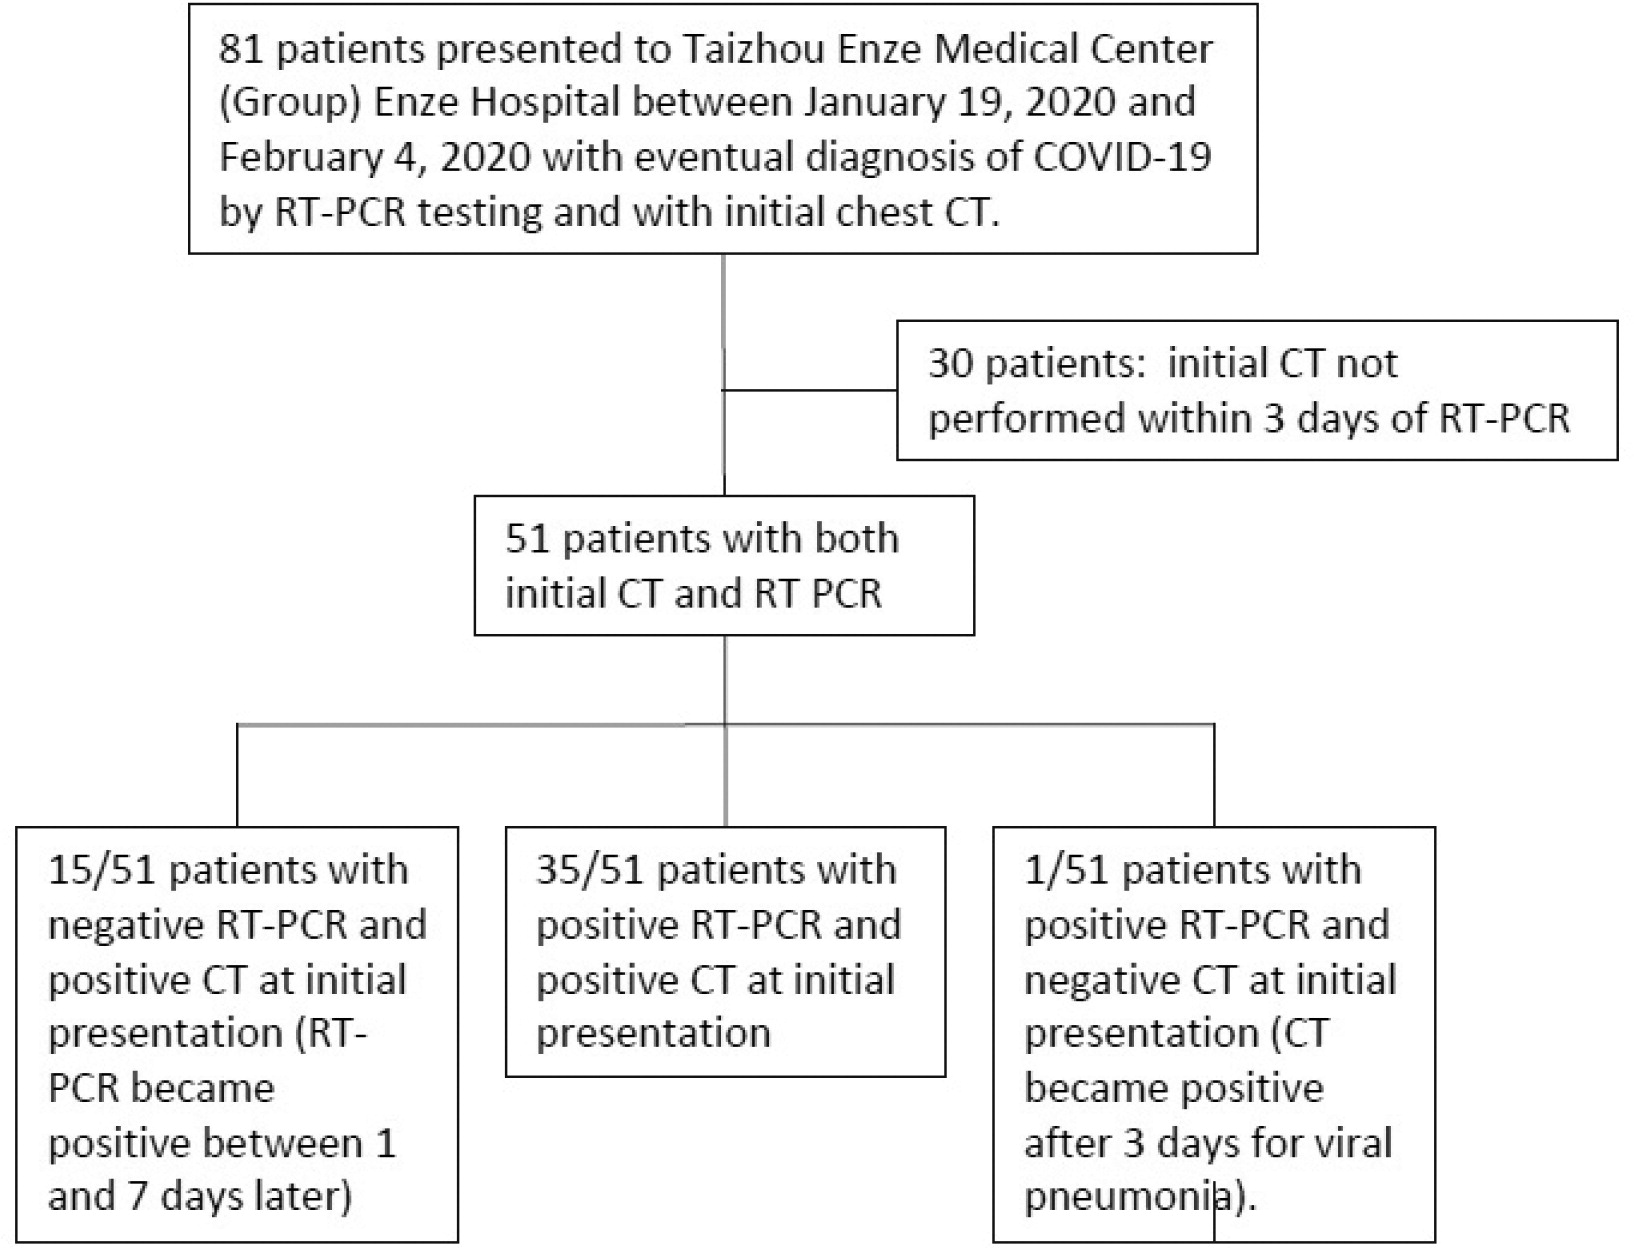
\includegraphics[width=8cm]{figures/RT_PCR_sensitivity.jpeg}
  \captionof{figure}{Figure from [1], indicating a significantly higher false negative rate of RT-PCR compared to CT scan}
  \par
}

\section*{Acknowledgment}
We thank Dr. Zeqing Xu and Dr. Zhiqiang Zhang for helpful conversations.

\end{multicols}
\begin{thebibliography}{20}

\bibitem{PCR-1} Yicheng Fang et al, Sensitivity of Chest CT for COVID-19: Comparison to RT-PCR, Radiology, Published online Feb 19 2020 \url{https://pubs.rsna.org/doi/10.1148/radiol.2020200432}

\bibitem{PCR-2} Xingzhi Xie, et al, Chest CT for Typical 2019-nCoV Peeumonia: Relationshop to Negative RT-PCR Tesing, Radiology, Published Online: Feb 12 2020 \url{https://pubs.rsna.org/doi/10.1148/radiol.2020200343}

\bibitem{CT1} Ai T, Yang Z, Hou H, Zhan C, Chen C, Lv W, Tao Q, Sun Z, Xia L. Correlation of Chest CT and RT-PCR Testing in Coronavirus Disease 2019 (COVID-19) in China: A Report of 1014 Cases. Radiology 2020:200642. doi: 10.1148/radiol.2020200642

\bibitem{CT2} Heshui Shi et al, Radiological findings from 81 patients with COVID-19 pneumonia in Wuhan, China: a descriptive study, The Lancet, \url{https://www.thelancet.com/article/S1473-3099(20)30086-4/fulltext}

\bibitem{CT3} Zi Yue Zu et al, Coronavirus Disease 2019 (COVID-19): A Perspective from China, Radiology, Published Online: Feb 21 2020 \url{https://pubs.rsna.org/doi/10.1148/radiol.2020200490}

\bibitem{use} Rubin, GD et al, The Role of Chest Imaging in Patient Management during the COVID-19 Pandemic: A Multinational Consensus Statement from the Fleischner Society,Radiology, Published online Apr 7 2020 \url{https://pubs.rsna.org/doi/10.1148/radiol.2020201365}

\bibitem{cost} \url{https://www.americanhealthimaging.com/how-much-does-a-ct-scan-cost/}
\end{thebibliography}

% \bibliography{MyCollection.bib}



\end{document}